\documentclass{beamer}

\usepackage{tikz}
\usetikzlibrary{positioning}

\title{Clean Architecture in .NET}
\author{Michal Gajda}
\institute{.NET - Liverpool Meetup}
\date{28 October 2025}

\begin{document}

\frame{\titlepage}

\begin{frame}
\frametitle{What is Clean Architecture?}
{\bfseries Clean Architecture} is an {\bfseries architecture pattern} aimed at building applications that we can maintain, scale, and test easily.
\\
It achieves this by separating the application into different layers that have distinct responsibilities.
\end{frame}

\begin{frame}
\frametitle{Reference vs Visibility Directions}
\centering

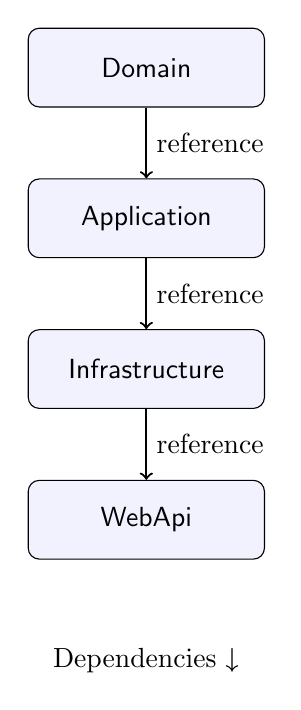
\begin{tikzpicture}[
  node distance=0.9cm,
  class/.style={rectangle, draw, rounded corners, fill=blue!5,
                minimum width=3cm, minimum height=1cm, font=\sffamily},
  arrow/.style={->, thick}
]
\node[class] (domain) {Domain};
\node[class, below=of domain] (application) {Application};
\node[class, below=of application] (infrastructure) {Infrastructure};
\node[class, below=of infrastructure] (webapi) {WebApi};

\draw[arrow] (domain.south) -- node[right]{reference} (application.north);
\draw[arrow] (application.south) -- node[right]{reference} (infrastructure.north);
\draw[arrow] (infrastructure.south) -- node[right]{reference} (webapi.north);

\node[below=1cm of webapi] {Dependencies ↓};
\end{tikzpicture}
\hspace{1cm}
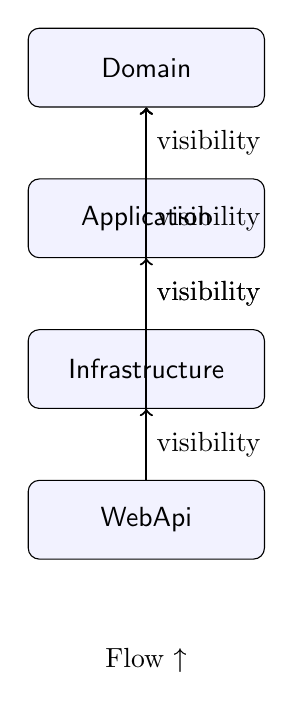
\begin{tikzpicture}[
  node distance=0.9cm,
  class/.style={rectangle, draw, rounded corners, fill=blue!5,
                minimum width=3cm, minimum height=1cm, font=\sffamily},
  arrow/.style={<-, thick} % zmieniony kierunek strzałek
]
\node[class] (domain2) {Domain};
\node[class, below=of domain2] (application2) {Application};
\node[class, below=of application2] (infrastructure2) {Infrastructure};
\node[class, below=of infrastructure2] (webapi2) {WebApi};

\draw[arrow] (domain2.south) -- node[right]{visibility} (application2.north);
\draw[arrow, shift={(0.3cm,0.2cm)}] (domain2.south) -- node[right]{visibility} (infrastructure2.north);
\draw[arrow] (domain2.south) -- node[right]{visibility} (webapi2.north);
\draw[arrow] (application2.south) -- node[right]{visibility} (infrastructure2.north);
\draw[arrow] (infrastructure2.south) -- node[right]{visibility} (webapi2.north);

\node[below=1cm of webapi2] {Flow ↑};
\end{tikzpicture}

\end{frame}

\begin{frame}
\frametitle{Dependencies vs Events}
\centering

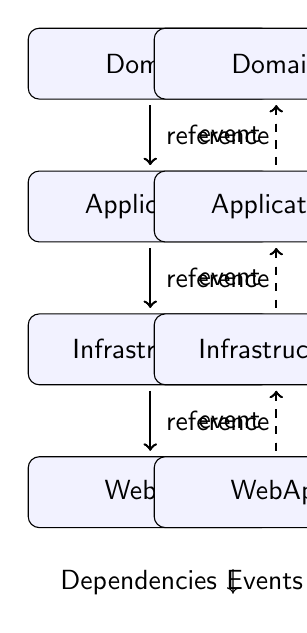
\begin{tikzpicture}[
  node distance=0.9cm,
  class/.style={rectangle, draw, rounded corners, fill=blue!5,
                minimum width=3.1cm, minimum height=0.9cm, font=\sffamily},
  ref/.style={->, thick, shorten >=2pt, shorten <=2pt},
  evt/.style={<-, thick, dashed, shorten >=2pt, shorten <=2pt}, % druga, „przesunięta” strzałka
  every node/.style={font=\sffamily}
]

% ====== LEWY SŁUPEK (strzałki w dół) ======
\node[class] (domain) {Domain};
\node[class, below=of domain] (application) {Application};
\node[class, below=of application] (infrastructure) {Infrastructure};
\node[class, below=of infrastructure] (webapi) {WebApi};

% Para strzałek między poziomami: „reference” + „event (offset 0.5cm)”
\draw[ref] (domain.south) -- node[right, xshift=2pt]{reference} (application.north);
\draw[ref, yshift=0.5cm] (domain.south) -- (application.north);

\draw[ref] (application.south) -- node[right, xshift=2pt]{reference} (infrastructure.north);
\draw[ref, yshift=0.5cm] (application.south) -- (infrastructure.north);

\draw[ref] (infrastructure.south) -- node[right, xshift=2pt]{reference} (webapi.north);
\draw[ref, yshift=0.5cm] (infrastructure.south) -- (webapi.north);

\node[below=4mm of webapi] {Dependencies ↓};

% ====== ODSTĘP MIĘDZY SŁUPKAMI ======
\hspace{1.6cm}

% ====== PRAWY SŁUPEK (strzałki w górę) ======
\node[class] (domain2) {Domain};
\node[class, below=of domain2] (application2) {Application};
\node[class, below=of application2] (infrastructure2) {Infrastructure};
\node[class, below=of infrastructure2] (webapi2) {WebApi};

% Para strzałek: w górę (odwrócone), druga przesunięta o 0.5cm
\draw[evt] (domain2.south) -- node[left, xshift=-2pt]{event} (application2.north);
\draw[evt, yshift=-0.5cm] (domain2.south) -- (application2.north);

\draw[evt] (application2.south) -- node[left, xshift=-2pt]{event} (infrastructure2.north);
\draw[evt, yshift=-0.5cm] (application2.south) -- (infrastructure2.north);

\draw[evt] (infrastructure2.south) -- node[left, xshift=-2pt]{event} (webapi2.north);
\draw[evt, yshift=-0.5cm] (infrastructure2.south) -- (webapi2.north);

\node[below=4mm of webapi2] {Events ↑};

\end{tikzpicture}
\end{frame}

\begin{frame}
\frametitle{How To Approach Clean Architecture Folder Structure?}
\end{frame}

\end{document}